% This file was created by tikzplotlib v0.8.5.
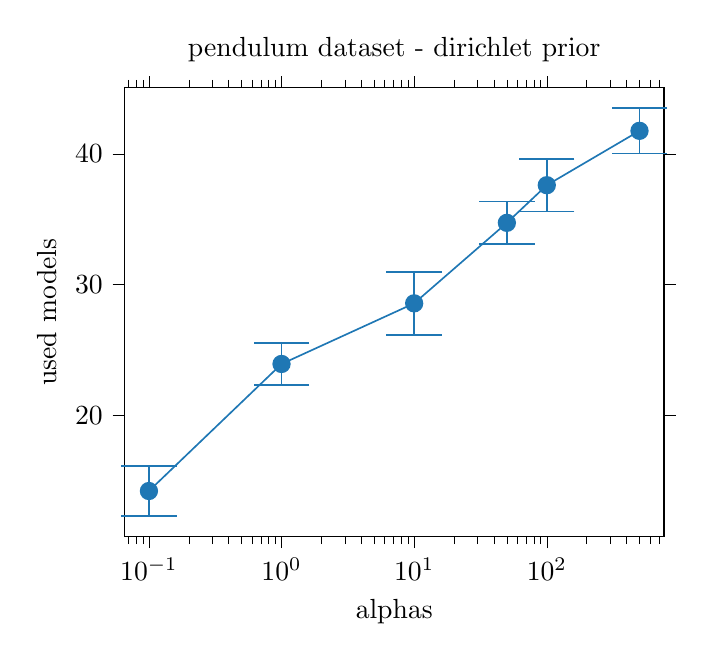
\begin{tikzpicture}

\definecolor{color0}{rgb}{0.12156862745098,0.466666666666667,0.705882352941177}

\begin{axis}[
log basis x={10},
tick align=outside,
tick pos=both,
title={pendulum dataset - dirichlet prior },
x grid style={white!69.01960784313725!black},
xlabel={alphas},
xmin=0.0653208007180445, xmax=765.452956031932,
xmode=log,
xtick style={color=black},
y grid style={white!69.01960784313725!black},
ylabel={used models},
ymin=10.7434169415142, ymax=45.0461791139786,
ytick style={color=black}
]
\path [draw=color0, semithick]
(axis cs:0.1,12.302633403899)
--(axis cs:0.1,16.097366596101);

\path [draw=color0, semithick]
(axis cs:1,22.2971629779919)
--(axis cs:1,25.5428370220081);

\path [draw=color0, semithick]
(axis cs:10,26.1586670368314)
--(axis cs:10,30.9613329631686);

\path [draw=color0, semithick]
(axis cs:50,33.0824408407633)
--(axis cs:50,36.3575591592367);

\path [draw=color0, semithick]
(axis cs:100,35.5800990123276)
--(axis cs:100,39.6199009876724);

\path [draw=color0, semithick]
(axis cs:500,40.0330373484062)
--(axis cs:500,43.4869626515938);

\addplot [semithick, color0, mark=-, mark size=10, mark options={solid}, only marks]
table {%
0.1 12.302633403899
1 22.2971629779919
10 26.1586670368314
50 33.0824408407633
100 35.5800990123276
500 40.0330373484062
};
\addplot [semithick, color0, mark=-, mark size=10, mark options={solid}, only marks]
table {%
0.1 16.097366596101
1 25.5428370220081
10 30.9613329631686
50 36.3575591592367
100 39.6199009876724
500 43.4869626515938
};
\addplot [semithick, color0, mark=*, mark size=3, mark options={solid}]
table {%
0.1 14.2
1 23.92
10 28.56
50 34.72
100 37.6
500 41.76
};
\end{axis}

\end{tikzpicture}
